\title{21. Vztahy geometrických útvarů v rovině - podobnost a stejnolehlost}
\author{Jonáš Lavička}
\date{1.5.2025}

\maketitle

\section{Vztahy geometrických útvarů v rovině\\- podobnost a stejnolehlost}
    \subsection{Definice}
        Dva geometrické útvary nazýváme podobné, jestliže poměry délek všech dvojic odpovídajících si úseček těchto útvarů se rovnají témuž číslu - koeficientu podobnosti.\\
        Podobnost zachovává velikost úhlů a poměr délek.\\
        → Podobné útvary mají stejný tvar(bez ohledu na velikost)
        
    \subsection{Koeficient podobnosti}
        Koeficient podobnosti je poměr vzdálenosti dvou bodů daného geometrického útvaru a vzdálenosti. odpovídajících dvou bodů jiného geometrického útvaru.\\
        Rovinné útvary $O_{1}$ a $O_{2}$ jsou podobné, píšeme:  $O_{1} \sim O_{2}$\\
        Vyjádření poměru podobnosti: $k = \left| X'Y' \right|:\left| XY \right| = \frac{\left| X'Y' \right|}{\left| XY \right|}$ ; $\left| X'Y' \right| = k \cdot \left| XY \right|$

    \subsection{Zvětšení - zmenšení}
        \begin{align*}
            & k>1   && \Rightarrow \text{podobný útvar je zvětšený}\\
            & 0<k<1 && \Rightarrow \text{podobný útvar je zmenšený}\\
            & k=1   && \Rightarrow \text{útvar je shodný}
        \end{align*}

    \subsection{Podobnost trojúhelníka}
        Trojúhelníky $\bigtriangleup ABC$ a $\bigtriangleup DEF$ jsou si podobné (píšeme $\bigtriangleup ABC \sim \bigtriangleup DEF$), pokud vyhoví jedné z následujících vět:
        \subsubsection{Věta sss}
            Každé dva trojúhelníky, které mají sobě rovné poměry délek všech tří dvojic odpovídajících stran, jsou si podobné.\\
            \[k=\frac{\left| DE \right|}{\left| AB \right|}=\frac{\left| EF \right|}{\left| BC \right|}=\frac{\left| DF \right|}{\left| AC \right|} \;\;\; \equiv \;\;\; k=\frac{a}{d}=\frac{b}{e}=\frac{c}{f}\]

            \begin{figure}[H]
                \centering
                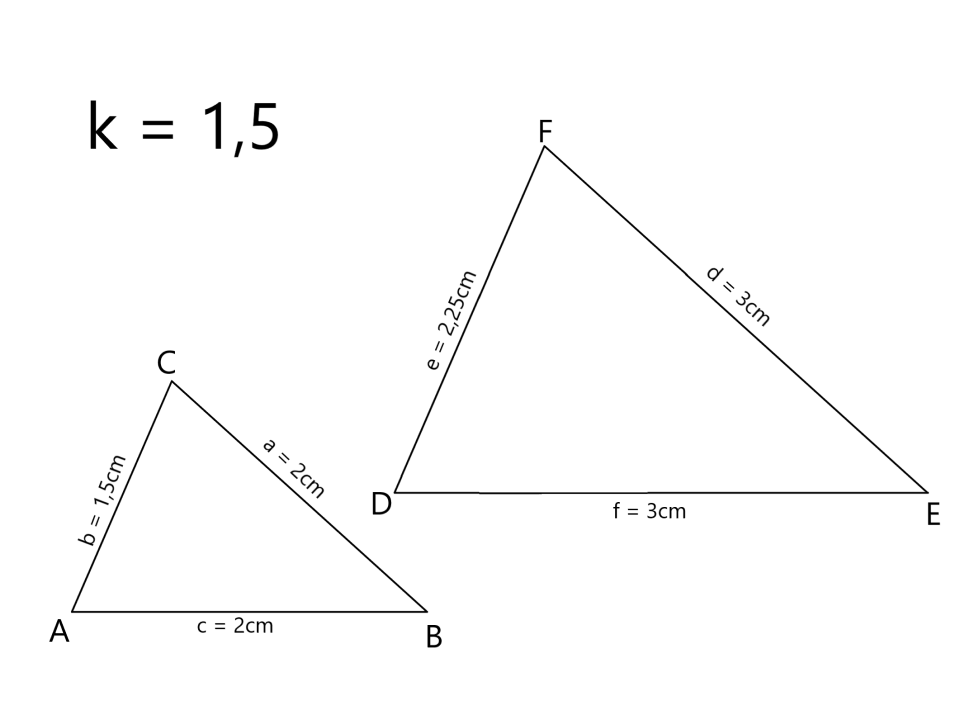
\includegraphics[width=0.5\linewidth]{img/23_trojuhelniky_sss.png}
                \caption{Podobné trojúhelníky dle věty sss} 
                \label{fig:enter-label}
            \end{figure}
            
        \subsubsection{Věta sus}
            Každé dva trojúhelníky, které mají sobě rovné poměry délek dvou odpovídajících stran a shodují se v úhlu jimi sevřeném, jsou si podobné.
            \[k=\frac{\left| DE \right|}{\left| AB \right|}=\frac{\left| DF \right|}{\left| AC \right|} \;\;\; \cap \;\;\; \left| \measuredangle BAC\right| = \left| \measuredangle EDF \right|\]

            \begin{figure}[H]
                \centering
                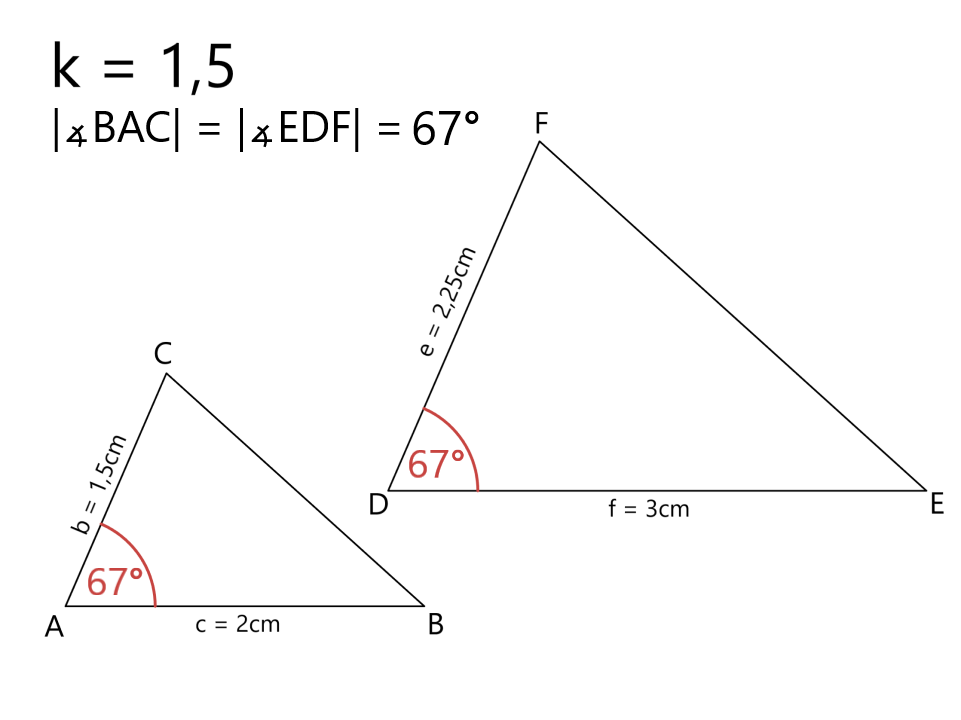
\includegraphics[width=0.5\linewidth]{img/23_trojuhelniky_sus.png}
                \caption{Podobné trojúhelníky dle věty sus} 
                \label{fig:enter-label}
            \end{figure}
            
        \subsubsection{Věta uu}
            Každé dva trojúhelníky, které mají dva úhly stejné, jsou si podobné.\\
            
            \begin{figure}[H]
                \centering
                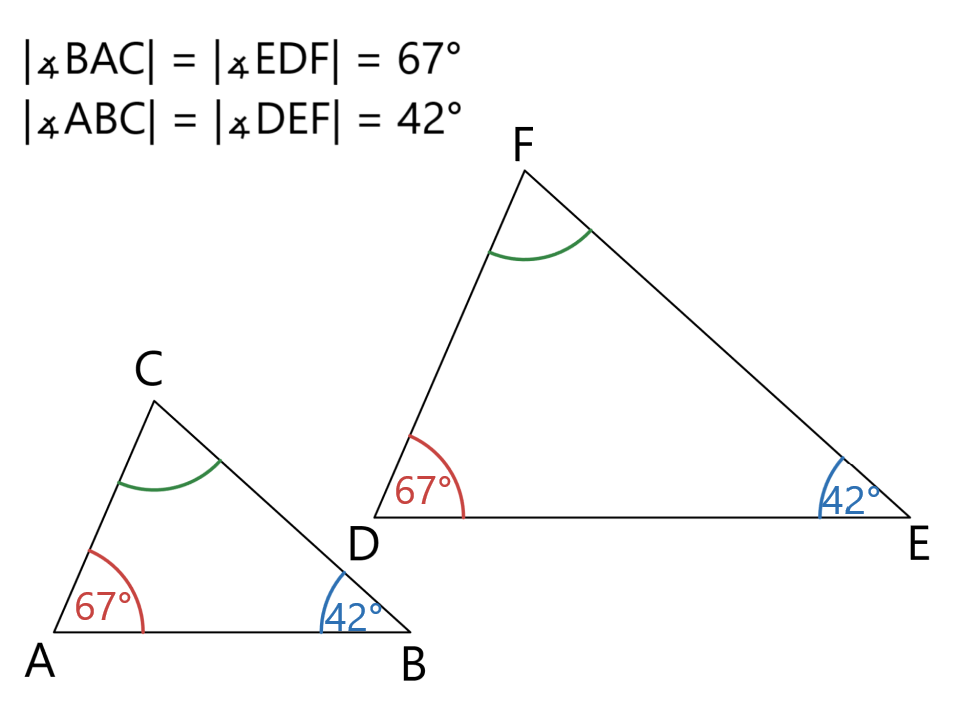
\includegraphics[width=0.5\linewidth]{img/23_trojuhelniky_uu.png}
                \caption{Podobné trojúhelníky dle věty uu} 
                \label{fig:enter-label}
            \end{figure}

        \subsubsection{Věta Ssu}
            Každé dva trojúhelníky, které mají sobě rovné poměry délek dvou odpovídajících stran a shodují se v úhlu naproti větší straně, jsou si podobné. Tento úhel je ostrý.
            \[k=\frac{\left| DE \right|}{\left| AB \right|}=\frac{\left| DF \right|}{\left| AC \right|} \;\;\; \cap \;\;\; \left| \measuredangle ABC\right| = \left| \measuredangle DEF \right|\]
            
            \begin{figure}[H]
                \centering
                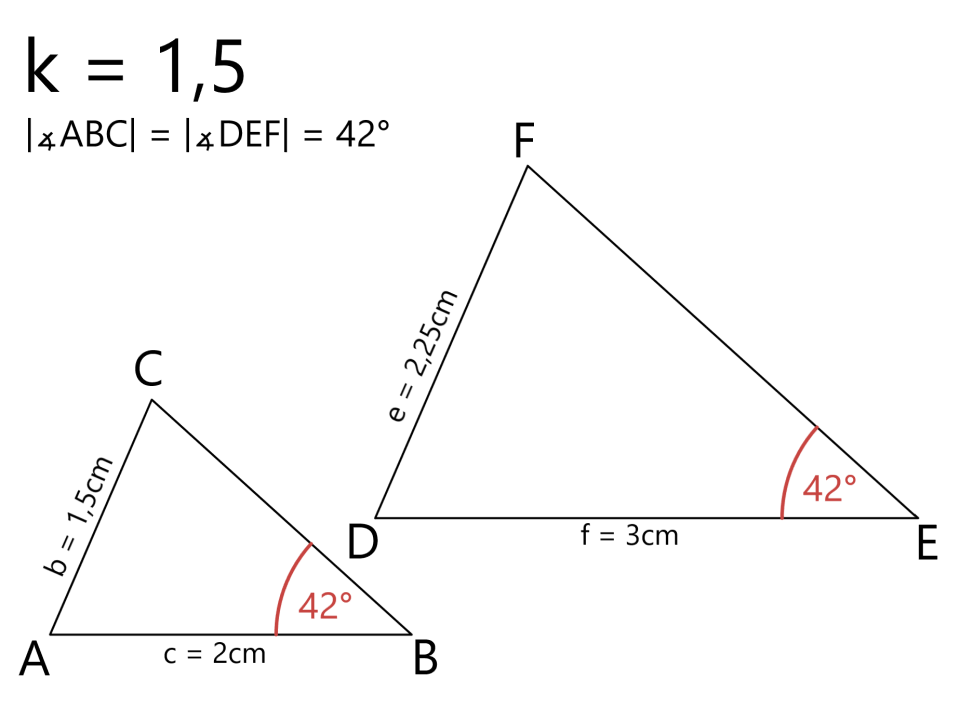
\includegraphics[width=0.5\linewidth]{img/23_trojuhelniky_Ssu.png}
                \caption{Podobné trojúhelníky dle věty Ssu} 
                \label{fig:enter-label}
            \end{figure}
    \newpage
    \subsection{Věty vyplývající z podobnosti trojúhleníků}
        \begin{itemize}
            \item Dva trojúhelníky jsou podobné, jsou-li jejich odpovídající si strany rovnoběžné, nebo navzájem kolmé.
            \item Dva pravoúhlé trojúhelníky jsou podobné, shodují-li se v jednom ostrém úhlu nebo v poměru dvou odpovídajících si stran.
            \item Dva rovnoramenné trojúhelníky jsou podobné, shodují-li se v úhlu při základně nebo v úhlu při vrcholu.
            \item Každé dva rovnostranné trojúhelníky jsou si podobné.
        \end{itemize}
    
    \subsection{Stejnolehlost}
        Stejnolehlost neboli homotetie $H(S,\kappa)$ je podobné zobrazení určené bodem $S$ a nenulovým reálným číslem - koeficientem stejnolehlosti $\kappa$, ve kterém se zobrazí bod $X \neq S$ na bod $X'$ tak, že: $\left| X'S \right| = \left| \kappa \right| \cdot \left| XS \right|$\\
        Pro $\kappa > 0$ bod $X'$ leží na polopřímce $\mapsto SX$.\\
        Pro $\kappa < 0$ bod $X'$ leží na polopřímce opačné k $\mapsto SX$.\\

        \begin{figure}[H]
            \centering
            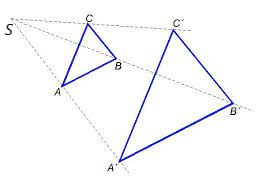
\includegraphics[width=0.5\linewidth]{img/23_stejnolehlost.png}
            \caption{Stejnolehlost s $\kappa>1$} 
            \label{fig:enter-label}
        \end{figure}
        
        Pro stejnolehlé zobrazení platí:
        \begin{itemize}
            \item Obrazem přímky je vždy přímka s ní rovnoběžná.
            \item Absolutní hodnota koeficientu stejnolehlosti je rovna koeficientu podobnosti.\\ $|\kappa| = k$
            \item $S$ Je samodružný bod. $S=S'$
            \item Pro koeficient stejnolehlosti roven $-1$ se jedná o středovou souměrnost, obraz je shodný, otočený o 180°.
        \end{itemize}

    \subsection{Eukleidovy věty}
        Eukleidovy věty se označují matematické věty o délkách odvěsen a výšky pravoúhlého trojúhelníku. Jsou to:
        \begin{itemize}
            \item Eukleidova věta o výšce: $v_c^2 = c_a \cdot c_b$
            \item Eukleidova věta o odvěsně: $a^2 = c \cdot c_a$
        \end{itemize}
        Podrobněji popsáno v otázce 24.